
Felten et al. (\citeyear{felten2021}) introduced the AIOE measure by linking ten AI applications to 52 O*NET abilities, 
using crowd-sourced relevance ratings to capture how strongly each application relates to a given ability. 
Summing these ratings yields an ability-level exposure score, $A_j$, where $j$ indexes the 52 abilities. 

Each job in O*NET also has ratings for how important and prevalent an ability is, denoted by $I_{jk}$ and $L_{jk}$ for job $k$. 
Since a job is essentially a weighted bundle of abilities, Felten et al. aggregate across them using 
$\sum_{j=1}^{52} L_{jk} \cdot I_{jk}$. 
To incorporate AI, they multiply by $A_j$ to capture how exposed each ability is to AI before summing across all abilities. 
The AIOE for some job $k$ is then: 
$$ \text{AIOE}_k = \frac{\sum_{j=1}^{52} A_j \cdot L_{jk} \cdot I_{jk}}{\sum_{j=1}^{52} L_{jk} \cdot I_{jk}}. $$ 

We validated our implementation by comparing our distribution of AIOE scores with the histogram reported by Felten et al. as done in Figure~\ref{fig:histograms}. 
While small differences arose from updated O*NET ratings, the overall shapes were consistent, suggesting fidelity to the original methodology. 

\begin{figure}[ht] 
    \centering 
    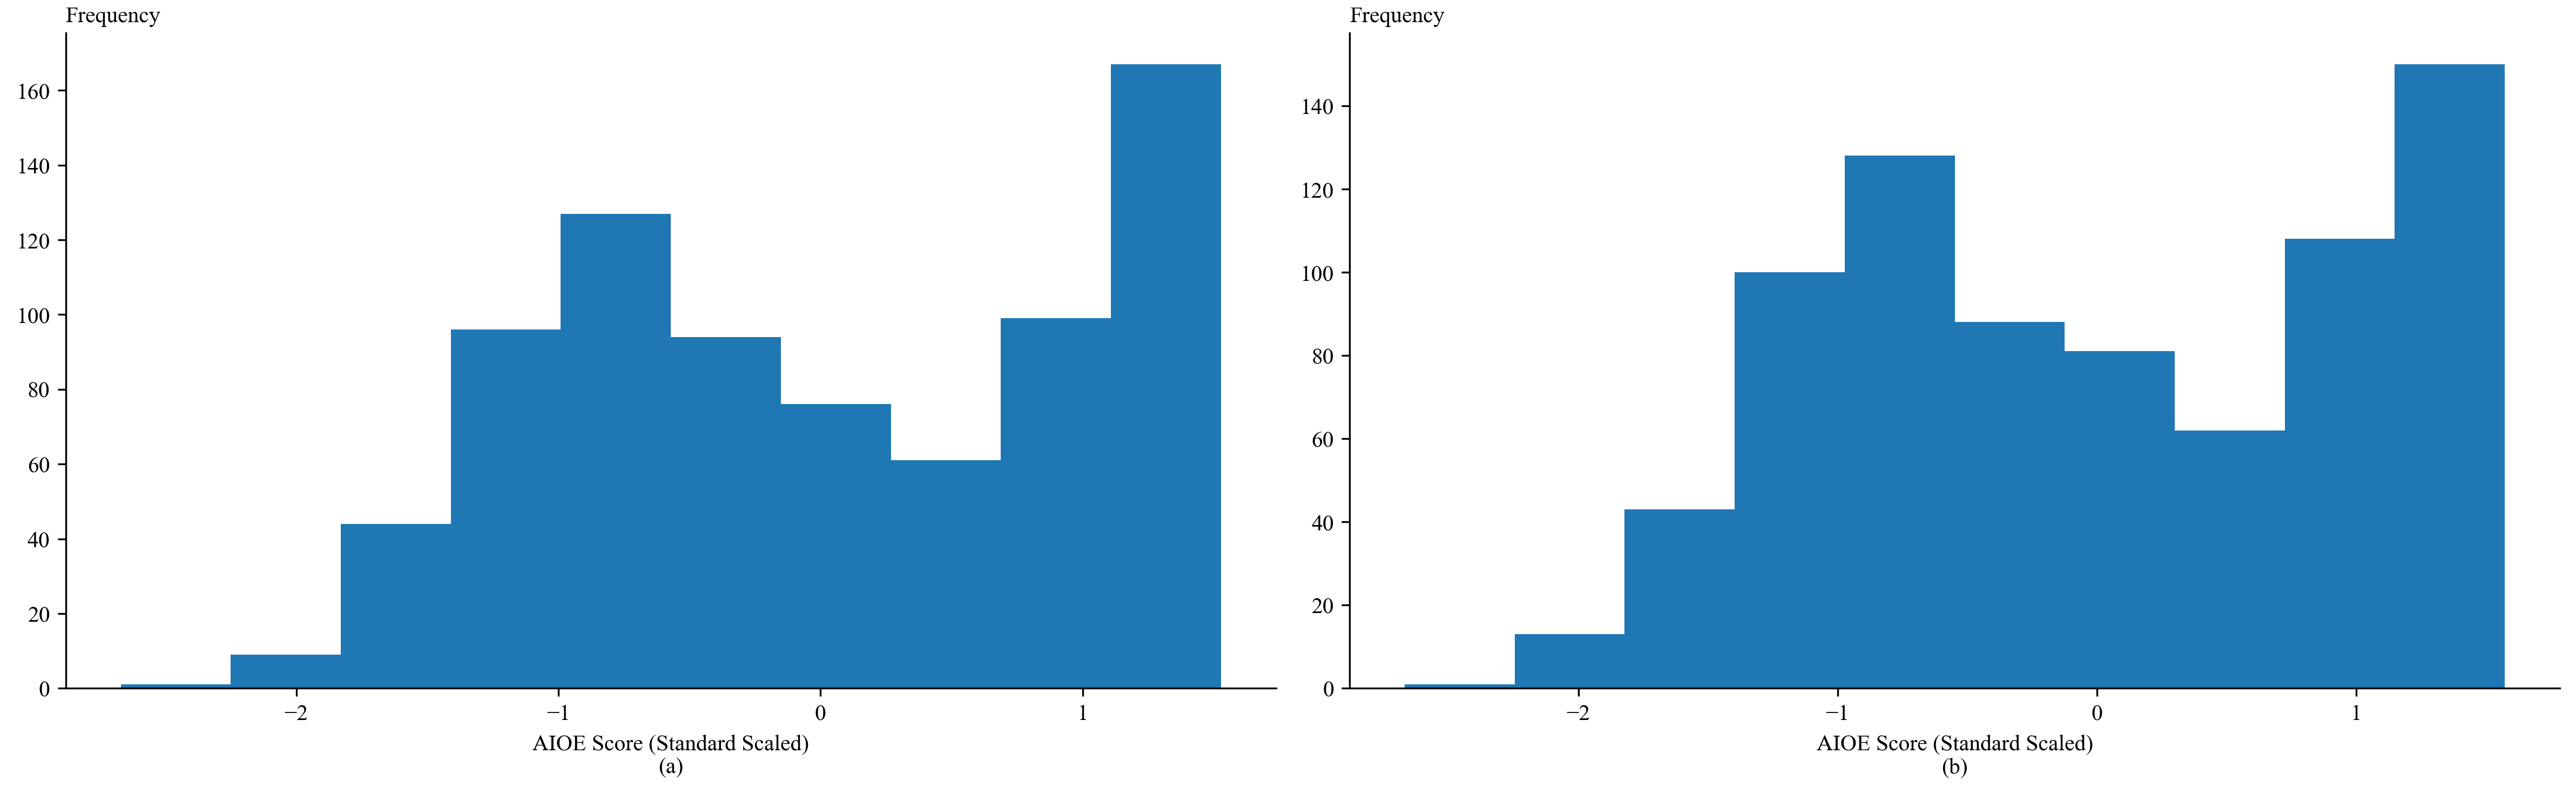
\includegraphics[width=\linewidth]{../figures/histograms_aioe.png} 
    \caption{Histograms of AIOE Scores by Felten et al. (a) and by Viray and Oximas (b)} 
    \label{fig:histograms} 
\end{figure} 

Some SOC codes did not directly map due to legacy classifications and were manually updated. 
Even after accounting for legacy codes, roughly 16.9\% of jobs lacked AIOE values, 
which we imputed using the median AIOE of their major-minor SOC group to account for the left-skewed distribution.